\documentclass[14pt]{beamer}

\usepackage{mathtools}
\usepackage{emoji}
\usepackage{xcolor}
\usepackage{xfrac}
\usepackage{csquotes}

\makeatother
\renewcommand{\thefootnote}{
    \ifcase\value{footnote}
        \or*
        \or**
        \or***
        \or****
    \fi}
\makeatletter

\usefonttheme{serif}
\setbeamertemplate{navigation symbols}{}%remove navigation symbols

\title{Scale independent font rasterization for interactive visualizations}
\author{Steffen Haug}
\date{}

\begin{document}
\begin{frame}
\titlepage
\end{frame}

\begin{frame}
    \centering
    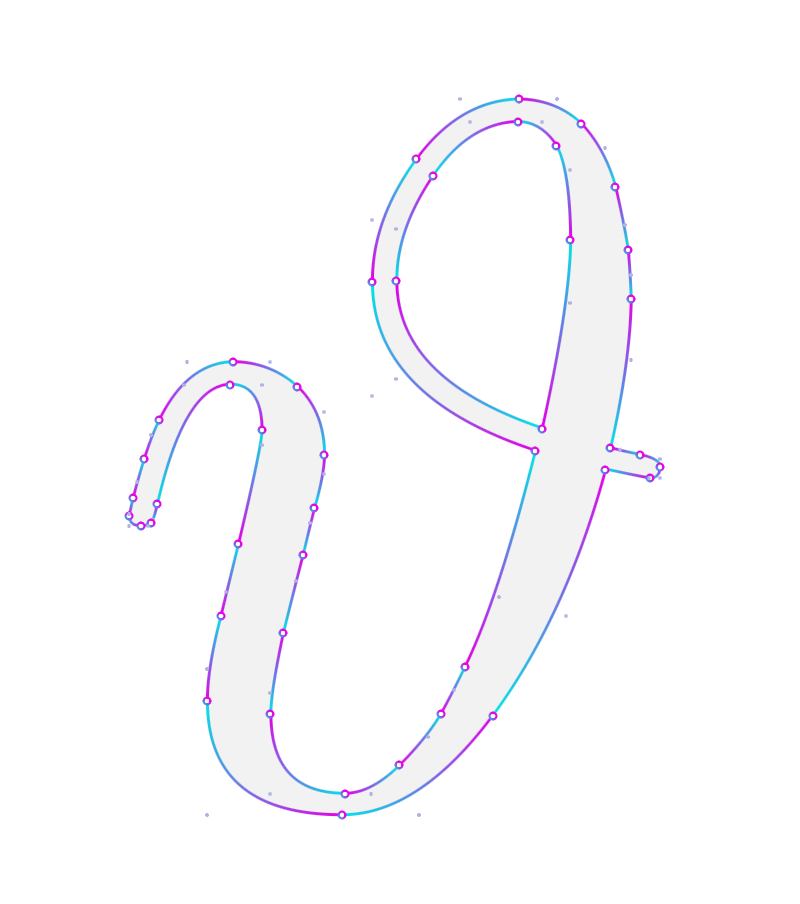
\includegraphics[width=0.625\textwidth]{demo/curves.png}

    How do we fill this in?
\end{frame}

\begin{frame}
    \centering
    My project implements a modified algorithm by Evan Wallace (2016) adjusted to
    deal with arbitrary number of self-intersections.
\end{frame}

\begin{frame}
    \centering
    Drawing the outline is actually easy!
\end{frame}

\begin{frame}
    \centering
    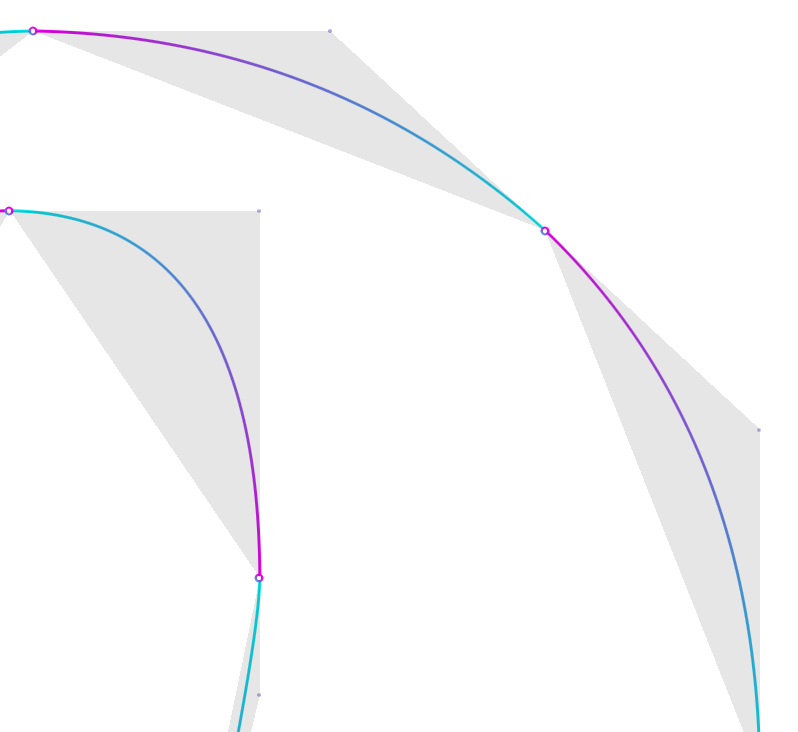
\includegraphics[height=0.625\textheight]{demo/loop_blinn_regions.png}

    Part of the glyph is contained in the convex hull of the control points.
\end{frame}

\begin{frame}
    \begin{itemize}
        \item<1-> Bézier curves defined by \textbf{linearly} interpolating between points.
        \item<2-> \textbf{Consequence:} We can just apply linear transformations to the control points.
        \item<3-> \textbf{Consequence:} We just have to find the inside in \textbf{one} coordinate system.
    \end{itemize}
    \pause
    \pause
    % By WE, of course, I mean somebody else
    Loop and Blinn (2005) already figured this out in the familiar $uv$-coordinates.
\end{frame}

\begin{frame}
    \centering
    Just put texture cordinates on the triangles!
    \begin{equation}
        u^2 - v > 0
    \end{equation}
\end{frame}

\begin{frame}
    \centering
    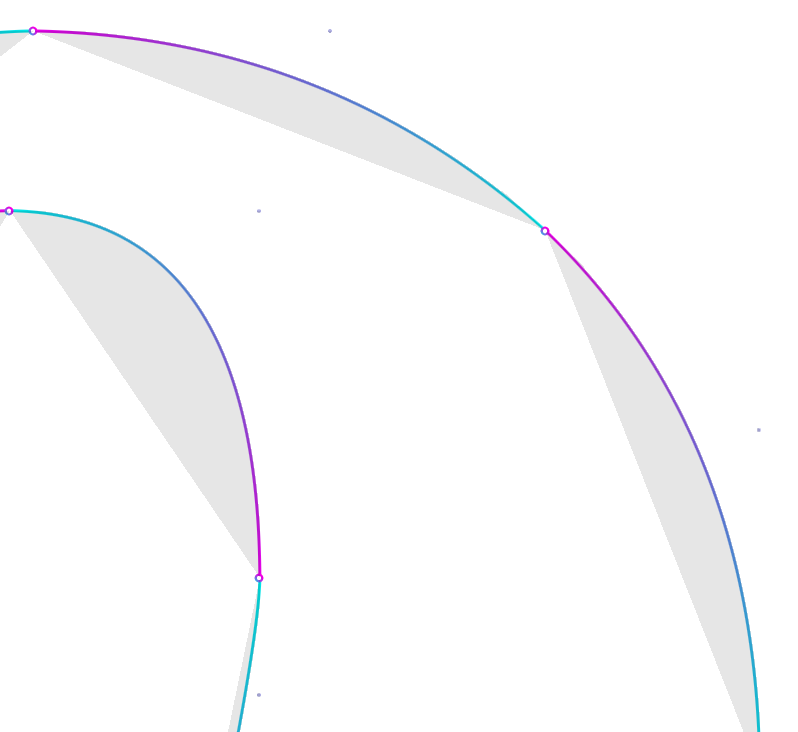
\includegraphics[height=0.625\textheight]{demo/outlines.png}

    Easy!
\end{frame}

\begin{frame}
    \centering
    Okay. So how do we fill the rest?
\end{frame}

\begin{frame}
    \begin{block}{Conjecture\!\footnote[1]{May very well be proved, I didn't check. (But it works!)}}
        We can add an auxillary point $P'$.
        If we extend the contour $C$ to visit $P'$ between line segments, we get a
        new (super-loopy) contour $C'$.
        The winding number $w$ of a fragment with respect to $C$ is the same as the
        winding number $w'$ with respect to $C'$ \textit{modolo two}:
        \begin{equation}
            w = w' \pmod 2
        \end{equation}
    \end{block}
\end{frame}

\begin{frame}
    \centering
    What?

    \Huge \emoji{face-with-raised-eyebrow}
    % not necessarily clear what this even means
    % DEFINITELY not clear how this helps
\end{frame}

\begin{frame}
    \centering
    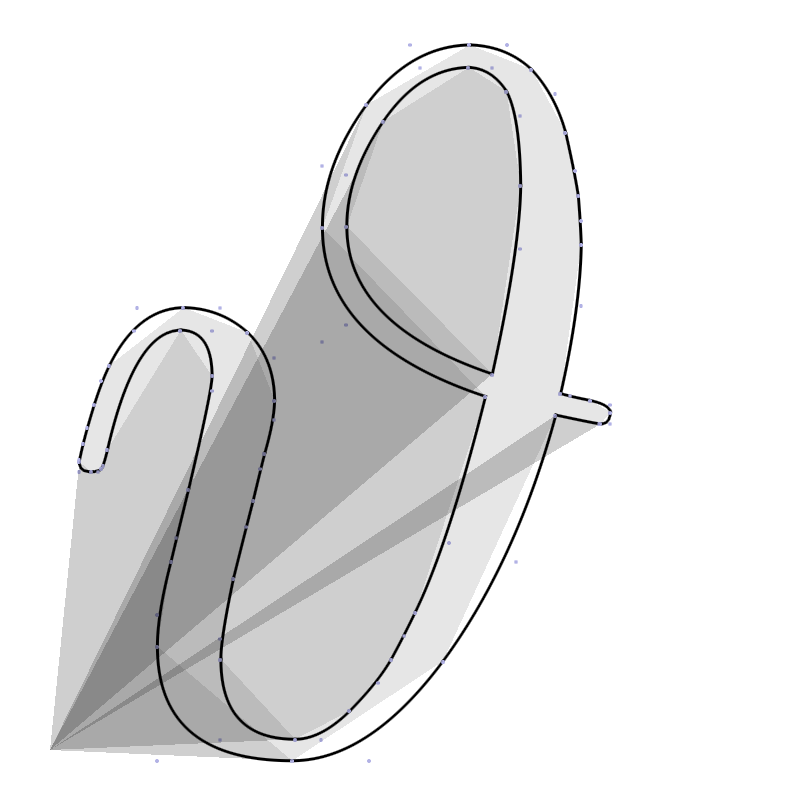
\includegraphics[height=0.625\textheight]{demo/step1.png}


    $$
    \mathtt{VertexID} = 1 \pmod 3  \implies \text{Send to zero}
    $$
\end{frame}

\begin{frame}
    \centering
    Not exactly clear how this helps...
\end{frame}

\begin{frame}
    \begin{itemize}
        \item<1-> The ``loops'' are \textbf{triangles}.
        \item<2-> Rasterizing a triangle \textbf{implicitly} calculates the winding number for that loop.
    \end{itemize}
    \pause
    Any shaded fragment was \textbf{inside} the triangle: I.~e. \textit{Contained in the loop once}.

    \centering\vspace{1.5em}
    Contribution of either $1$ or $0$ to $w'$!

    \vspace{1.5em}


    \begin{itemize}
        \item Repeat for every Bézier curve.
    \end{itemize}

\end{frame}

\begin{frame}
    \centering
    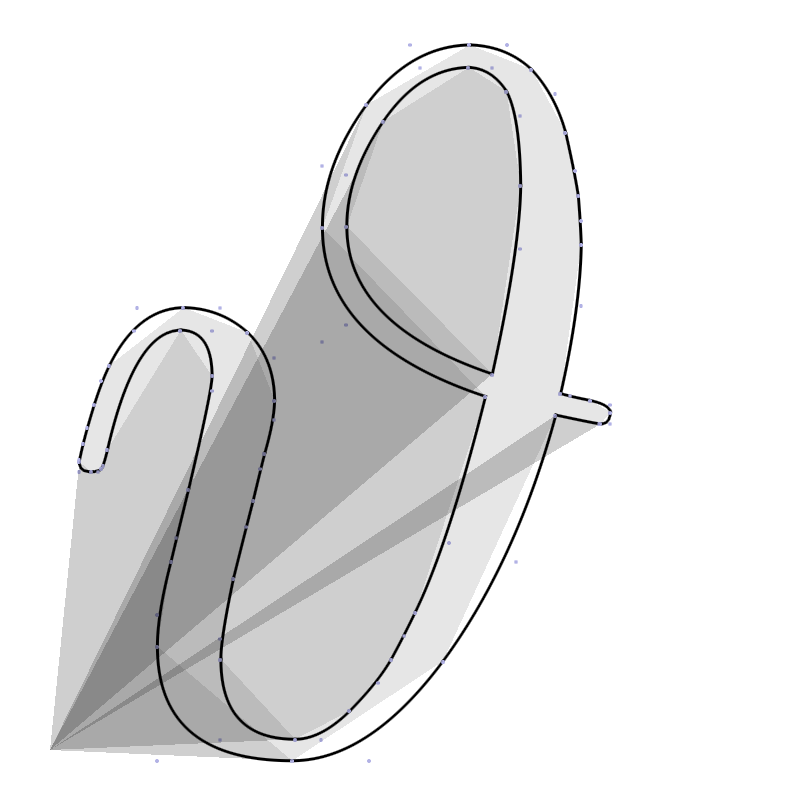
\includegraphics[height=0.625\textheight]{demo/step1.png}


    $w' = \text{Number of times rasterized to...}$
\end{frame}

\begin{frame}
    \centering
    $w' = \text{Number of times rasterized to...}$

    \vspace{1.5em}
    And $w = w' \pmod 2$

    \vspace{1.5em}
    \textit{How do we count this in a shader?}
\end{frame}

\begin{frame}
    Wallaces algorithm: \textbf{Shade with intensity \sfrac{1}{255}}.
    \begin{displayquote}
        ``The resulting pixel only lies inside the outline if the accumulated color scaled back up by 255 is odd.''
    \end{displayquote}
    \pause
    \textbf{Problem:} The contour is limited in the number of self-intersections.
\end{frame}

\begin{frame}
    \centering
    We don't have to count up $w'$ and \textbf{then} calculate the modulus.
\end{frame}

\begin{frame}
    \centering
    We should instead add modulo two \textbf{as we go}!

    \pause
    \vspace{1em}
    \begin{block}{Observation}
        Addition modulo two has the same identical table as logical XORs truth table:
        $$
        \begin{array}{c|cc}
              & 0 & 1 \\
            \hline
            0 & 0 & 1 \\
            1 & 1 & 0 \\ 
        \end{array}
        $$
        Minor point: Addition in this group is both assiciative and commutative.
        % i. e. we won't get a different result if we re-order the vertex buffer.
    \end{block}
\end{frame}

\begin{frame}
    \centering
    Three easy steps using an obscure OpenGL feature:
    \vspace{1em}


    \begin{itemize}
    \item Enable \texttt{gl::COLOR\_LOGIC\_OP} 
    \item Use operator \texttt{gl::XOR}.
    \item Draw the triangles
    \end{itemize}
\end{frame}

\begin{frame}
    \centering
    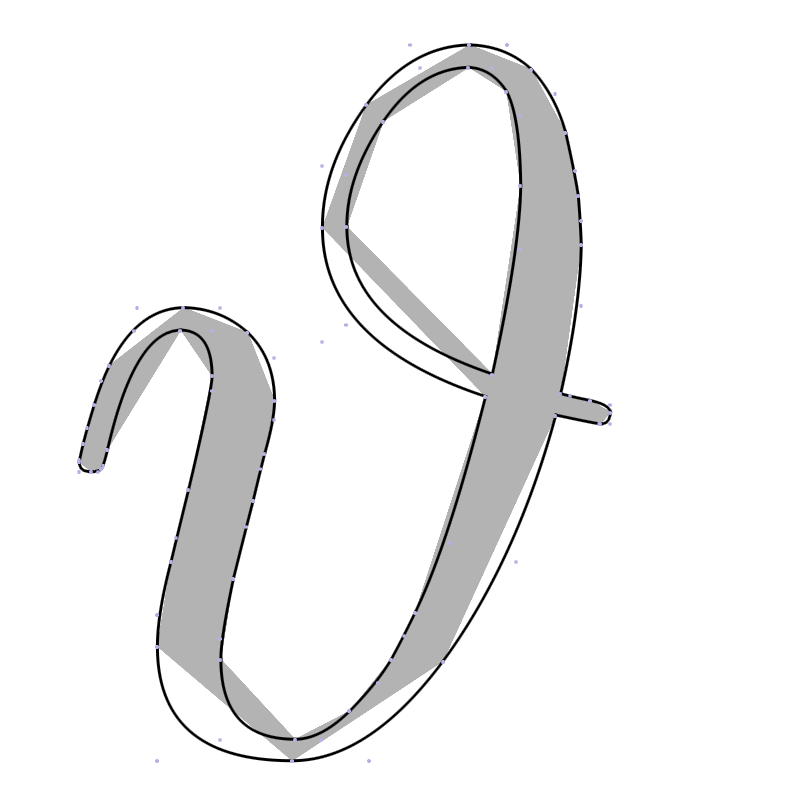
\includegraphics[height=0.625\textheight]{demo/step2.png}

    Approximation of the glyphs interior.

    \scriptsize{\quad}%just to align pic
\end{frame}

\begin{frame}
    \centering 
    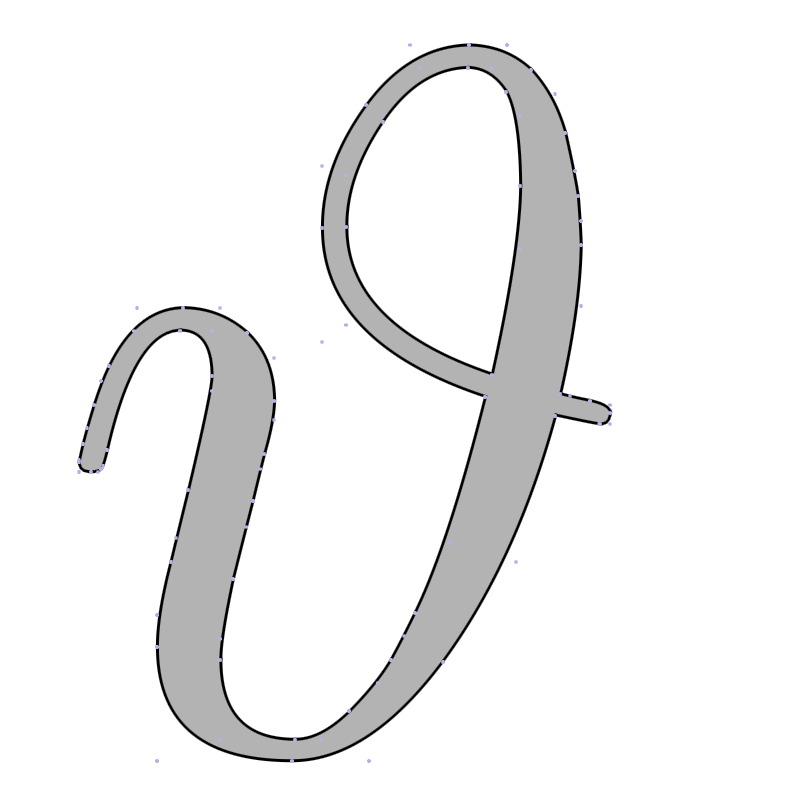
\includegraphics[height=0.625\textheight]{demo/step3.png}

    Fill in the outline regions.

    \scriptsize{(Still addition modulo two!)}
\end{frame}

\begin{frame}
    \centering 
    
\includegraphics[height=0.625\textheight]{demo/final.png}

    It works! Anti-aliasing with 16xMSAA.

    \scriptsize{\quad}%just to align pic
\end{frame}

\begin{frame}
    \frametitle{References}


    \begin{itemize}
        \item \textbf{Loop \& Blinn}: https://www.microsoft.com/en-us/research/wp-content/uploads/2005/01/p1000-loop.pdf

        \item \textbf{Wallace}: https://medium.com/@evanwallace/easy-scalable-text-rendering-on-the-gpu-c3f4d782c5ac
    \end{itemize}
\end{frame}


\end{document}
